%Preamble
\documentclass[aspectratio=43]{beamer}
\usepackage[english]{babel}
%Graphics
\usepackage{graphicx}
\graphicspath{{../images/}}
\usepackage[section]{placeins} %for FloatBarrier
\def\Put(#1,#2)#3{\leavevmode\makebox(0,0){\put(#1,#2){#3}}}
\usepackage{multicol}
%Refernces
\usepackage[natbib=true,
            bibencoding=utf8,
            style=authoryear,
            backend=biber,
            %autocite=superscript,
            sorting=none,
            useprefix=true]{biblatex}
\addbibresource{../refs.bib}

%Footnote
\newcommand\blfootnote[1]{%
    \begingroup
    \renewcommand\thefootnote{}\footnote{#1}%
    \addtocounter{footnote}{-1}%
    \endgroup
}

%Title
\title{\textbf{\Huge SELEXzyme} \\ \vspace{0.2in}Evolving DNAzymes for Target Sequences}
\subtitle{02-601 Project Presentation}
\author{Siddharth Reed}
\institute{Computational Biology Department \\ Carnegie Mellon University}
\date{\today}

\begin{document}
%Title
\frame{\titlepage}
\begin{frame}{Summary}
  \setbeamertemplate{section in toc}[sections numbered]
  \tableofcontents[hideallsubsections]
\end{frame}

\section{DNAzymes}
\begin{frame}[fragile]{What is a DNAzyme?}
\begin{columns}
    \begin{column}{0.5\textwidth}
        \begin{figure}[htb!]\onslide<2->
            \makebox[\textwidth][c]{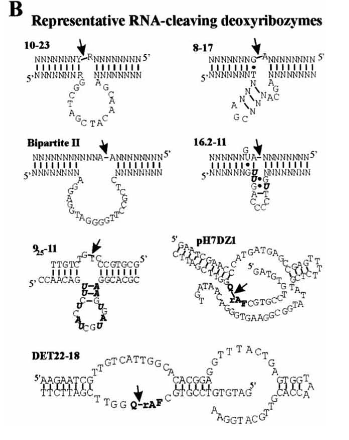
\includegraphics[width=\linewidth]{dnazyme.png}}
        \end{figure}
    \end{column}
    \begin{column}{0.5\textwidth}
        \begin{itemize}
            \item<2-> Short DNA sequences with catalytic activity
            \item<3-> Often cut target nucleotide sequences
            \item<4-> Can have tertiary structure
            \item<5-> Never before observed \textit{in vivo}
        \end{itemize}
    \end{column}
\end{columns}
\blfootnote{\cite{dnazyme}}
\end{frame}
\begin{frame}[fragile]{Why Care About DNAzymes?}
\begin{columns}
    \begin{column}{0.5\textwidth}
        \begin{figure}[htb!]\onslide<2->
            \makebox[\textwidth][c]{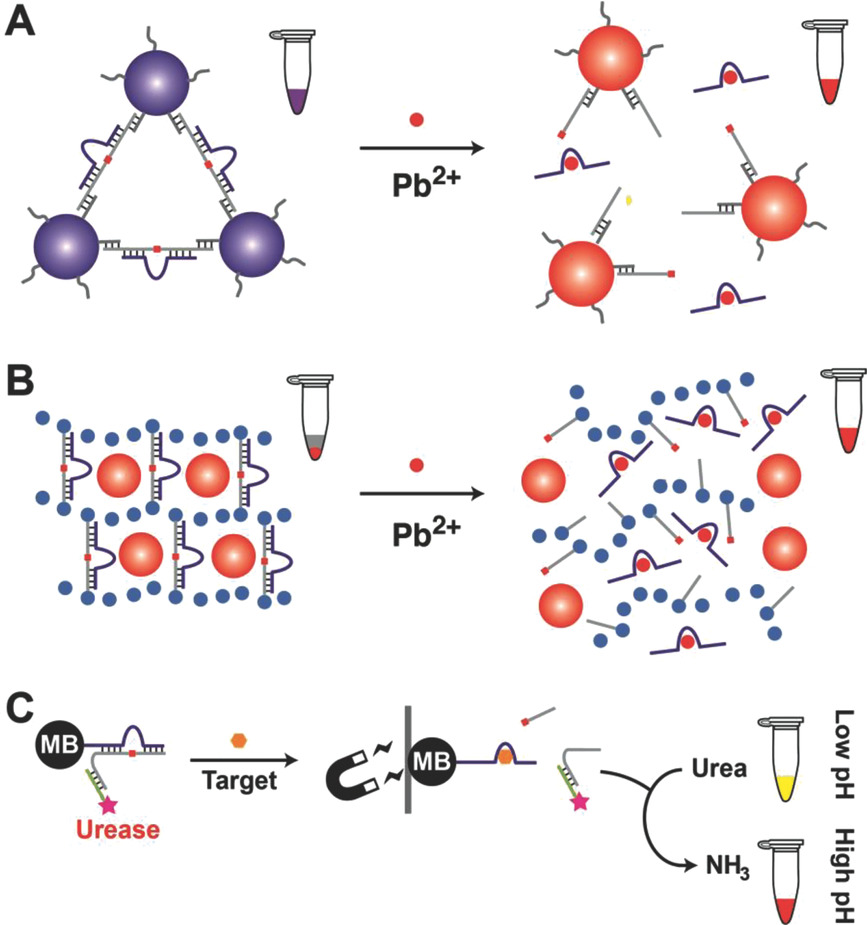
\includegraphics[width=0.8\linewidth]{color_sensor.jpg}}
        \end{figure}
    \end{column}
    \begin{column}{0.5\textwidth}
        \begin{itemize}
            \item<2-> Easy to synthesize, efficient production, highly active
            \item<3-> Chemical sensors, motors, therapeutics
            \item<4-> Can encode “logic” into DNAzyme constructs
            \item<5-> Often combined with DNA Aptamers i.e. DNA “antibodies”
        \end{itemize}
    \end{column}
\end{columns}
\blfootnote{\cite{apps};\cite{apps2}}
\end{frame}

\section{SELEX and Genetic Algorithms}
\begin{frame}[fragile]{How Do You Design DNAzymes?}
\begin{figure}[htb!]
    \makebox[\textwidth][c]{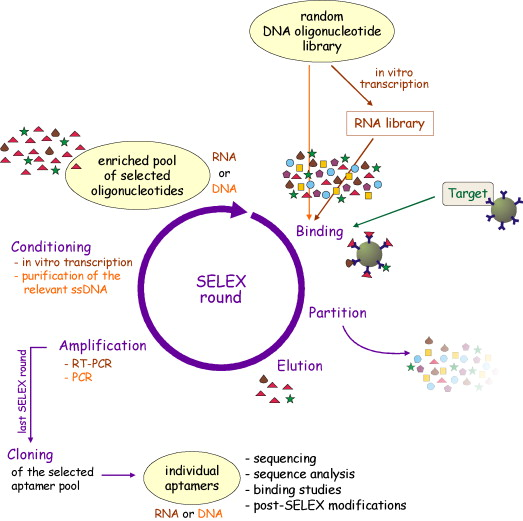
\includegraphics[width=0.7\linewidth]{selex.jpg}}
\end{figure}
\blfootnote{\cite{selex}}
\end{frame}
\begin{frame}[fragile]{Genetic Algorithms Simulate SELEX}
\begin{figure}[htb!]
    \makebox[\textwidth][c]{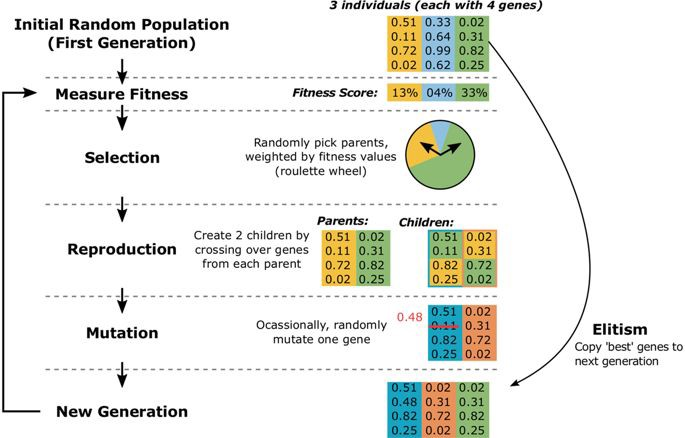
\includegraphics[width=\linewidth]{ga.jpg}}
\end{figure}
\blfootnote{\cite{ga_web}}
\end{frame}

\section{SELEXzyme}
\begin{frame}[fragile]{My Project}
\begin{itemize}
    \item<2-> GA to evolve possible DNAzymes that target a user-defined sequence
    \item<3-> Use a machine learning model to evaluate “DNAzyme-ness”
    \item<4-> GA built in Go, learning model trained with sk-learn
\end{itemize}
\begin{figure}[htb!]\onslide<5->
    \makebox[\textwidth][c]{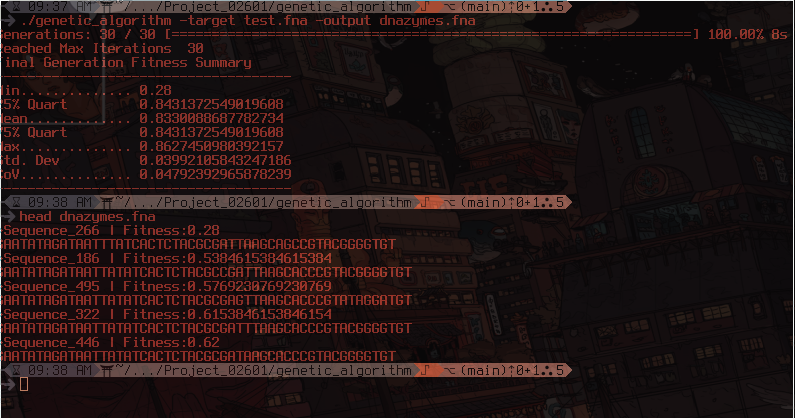
\includegraphics[width=0.8\linewidth]{output.png}}
\end{figure}
\end{frame}
\begin{frame}[fragile]{What is the Fitness Function?}
    \begin{itemize}
        \item<2-> Smith-Waterman alignment score to user target sequence
        \item<3-> Probability of being a DNAzyme from the ML model
        \item<4-> Use an SVM model, good for simplicity vs quality trade-off
        \item<5-> Model trained on known DNAzymes, DNA aptamers, Promoters and simulated data
    \end{itemize}
    \begin{figure}[htb!]\onslide<4->
        \makebox[\textwidth][c]{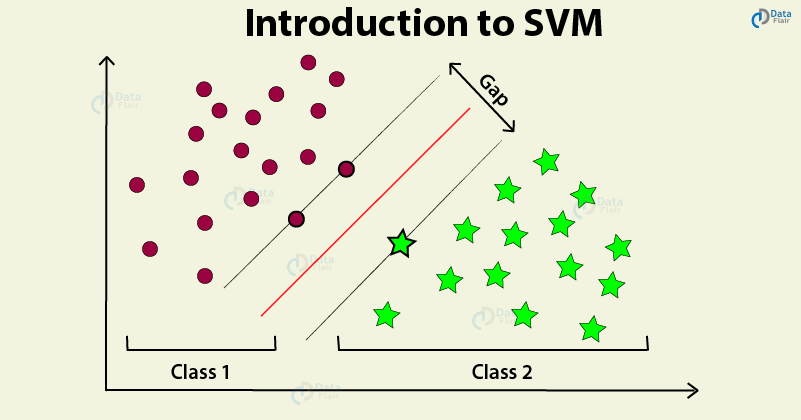
\includegraphics[width=0.8\linewidth]{svm.png}}
    \end{figure}
    \blfootnote{\cite{svm_dna};\cite{svm_pic}}
\end{frame}
\begin{frame}[fragile]{Validation}
\begin{figure}[htb!]
    \makebox[\textwidth][c]{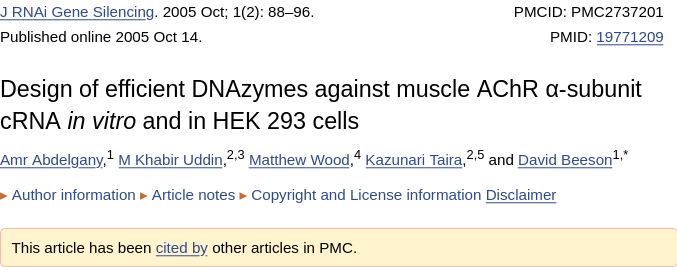
\includegraphics[width=0.9\linewidth]{validation.png}}
\end{figure}
\begin{itemize}
    \item<2-> Computationally generated vs. \textit{in vitro} screened DNAzymes
    \item<3-> Similar sequence composition (high alignment score)
    \item<4-> \textit{in vitro} screened DNAzymes should have high fitness values
\end{itemize}
\end{frame}

%Refs
\begin{frame}[allowframebreaks]{References}
    \printbibliography
\end{frame}
\end{document}


